\chapter*{Visualization}
In this section we provide an analysis of the data in terms of their
graphical representation and visualization. \\

\section*{Histograms}
We ploted a histogram for each attribute to investigate its distribution. 
Each histogram shows how many records had a value of attribute in a range
of particular bucket. \\
\begin{figure}[!tbh]
	\centering
	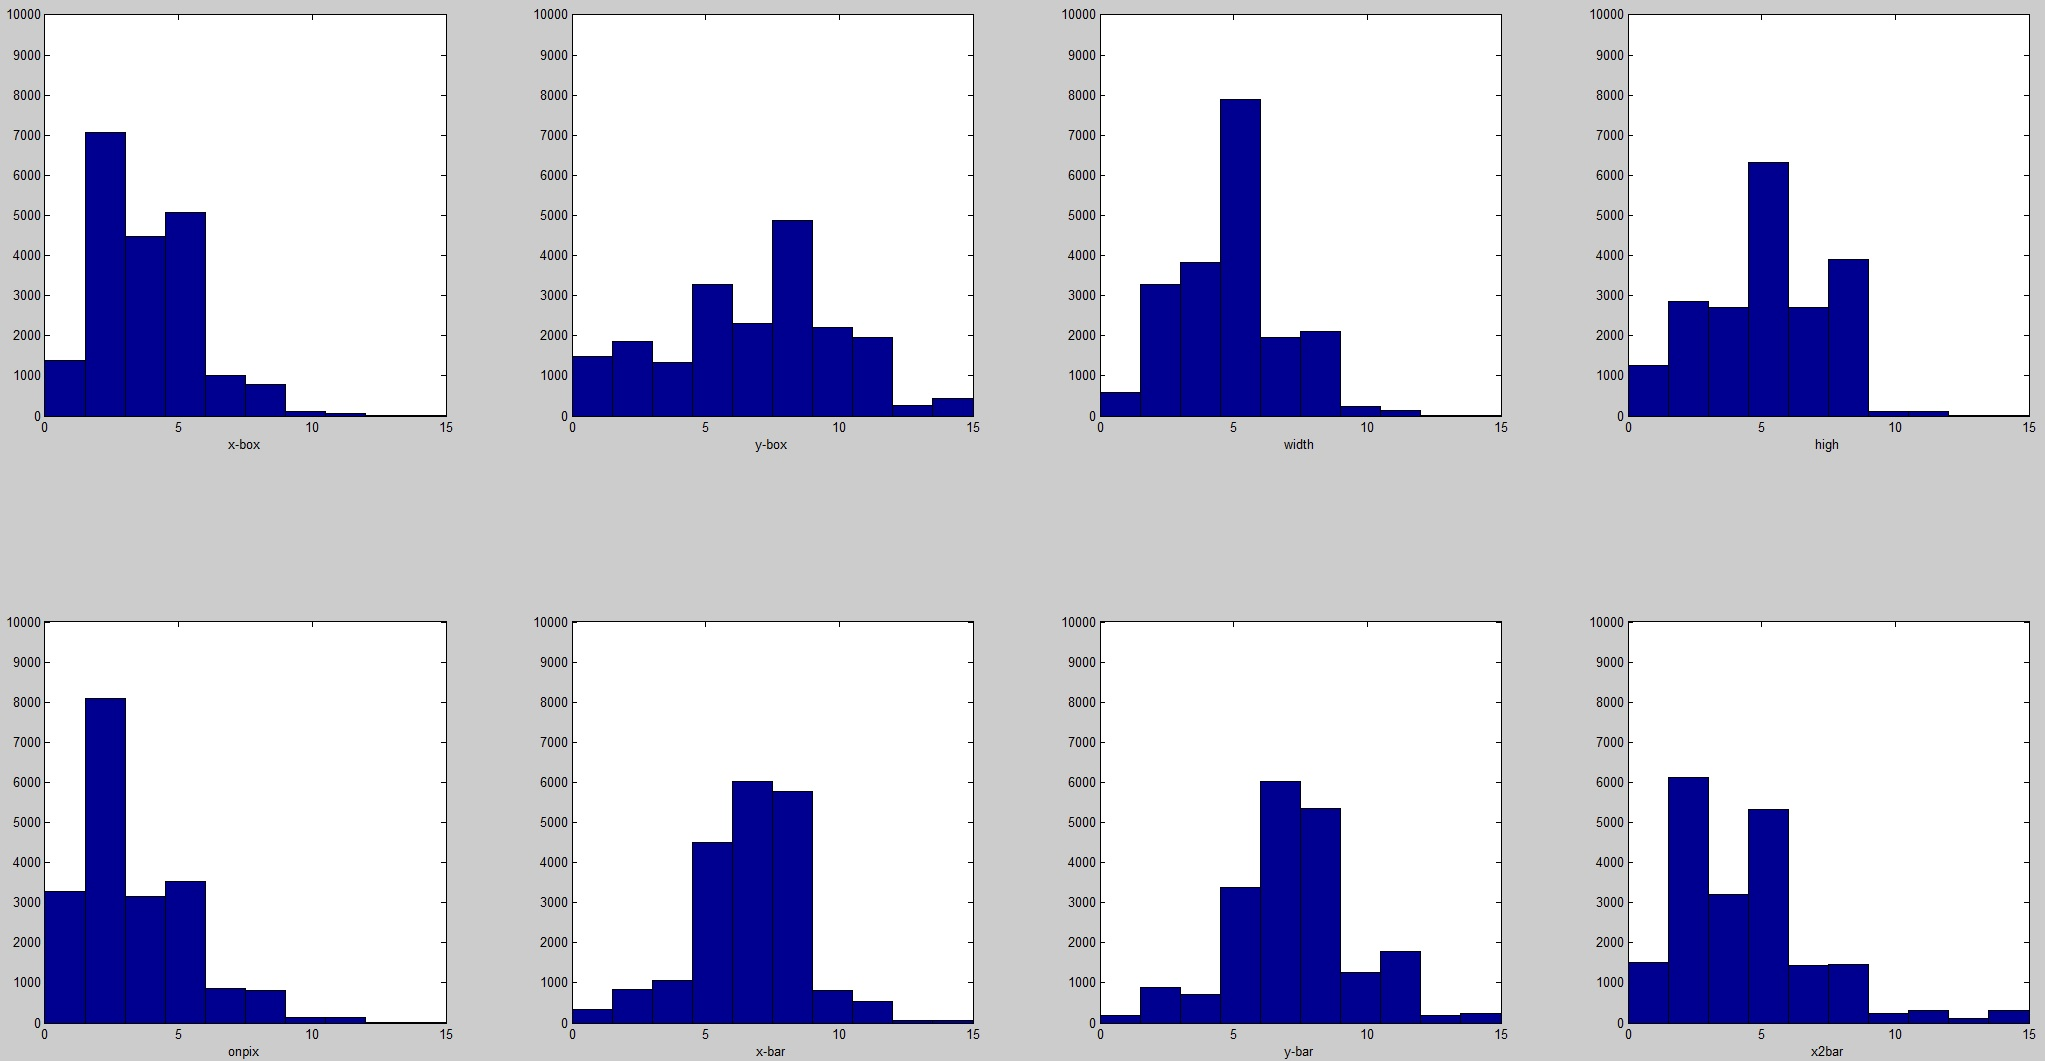
\includegraphics[width=0.8\textwidth]{figures/histograms_1}
	\caption{Histograms for first attributes 0-7}
	\label{fig:histograms_1}
\end{figure} 
\clearpage
We can notice that most of the attributes are normally distributed. \\
\begin{figure}[!tbh]
	\centering
	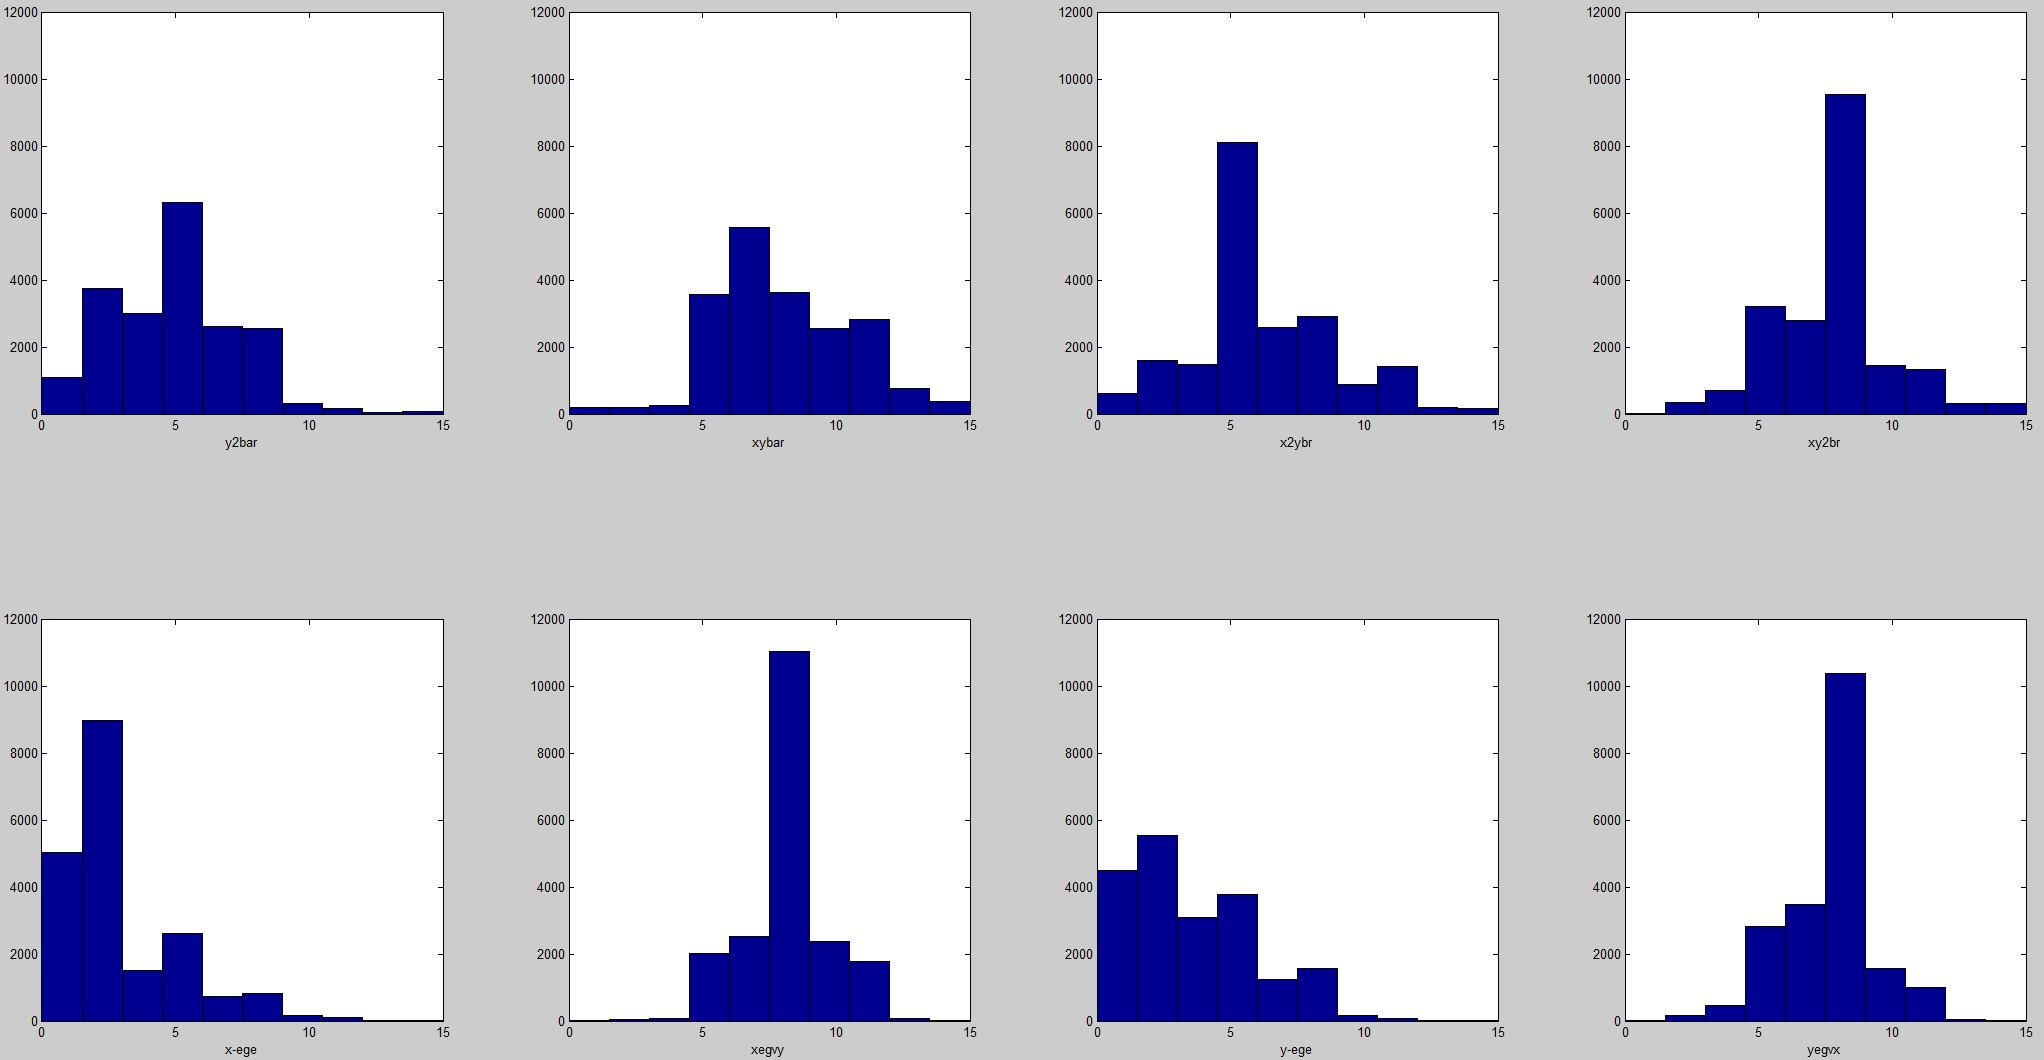
\includegraphics[width=0.8\textwidth]{figures/histograms_2}
	\caption{Histograms for first attributes 8-15}
	\label{fig:histograms_2}
\end{figure} 

\section*{Box plots}
We created box plot of our data in order to show the distribution of the
attribute values. We did it for all the records in dataset:
\begin{figure}[!tbh]
	\centering
	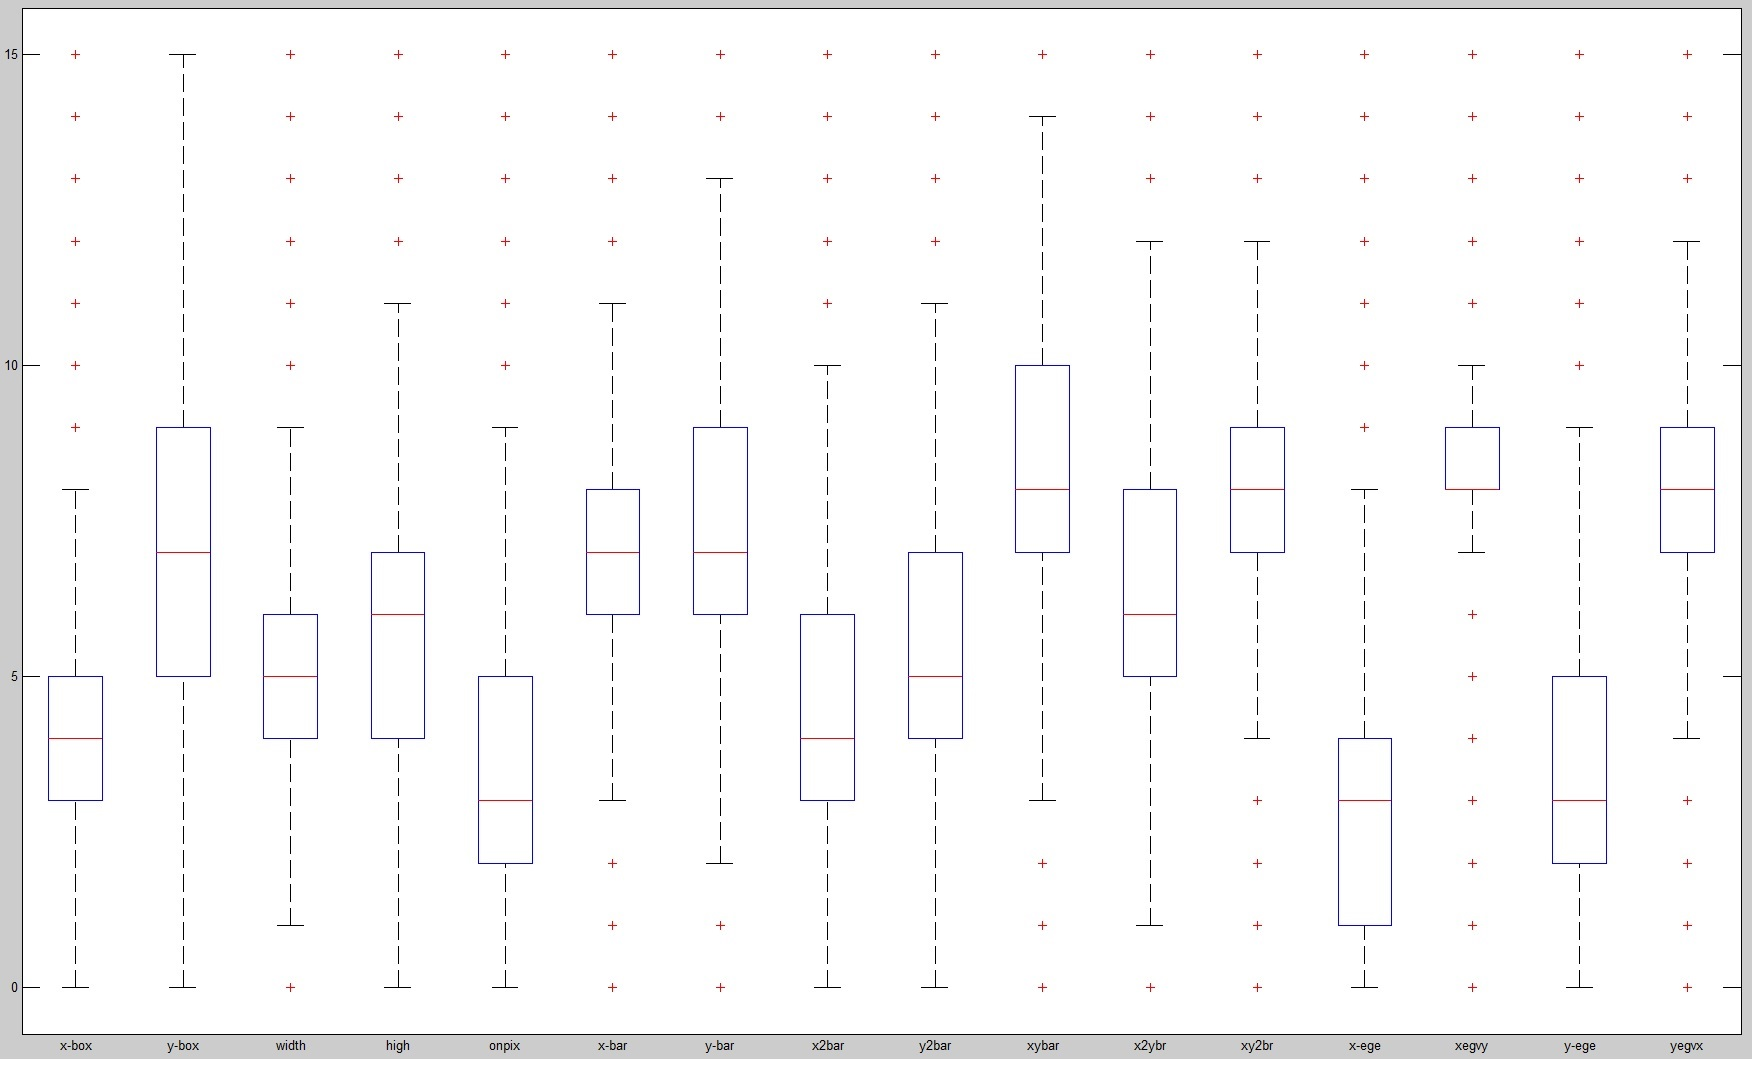
\includegraphics[width=0.9\textwidth]{figures/boxplot_all}
	\caption{Box plot for all records of the data set}
	\label{fig:boxplot_all}
\end{figure} \\
Also for first 3 classes (letter) to show how attributes differ from
one class to another: 
\begin{figure}[!tbh]
	\centering
	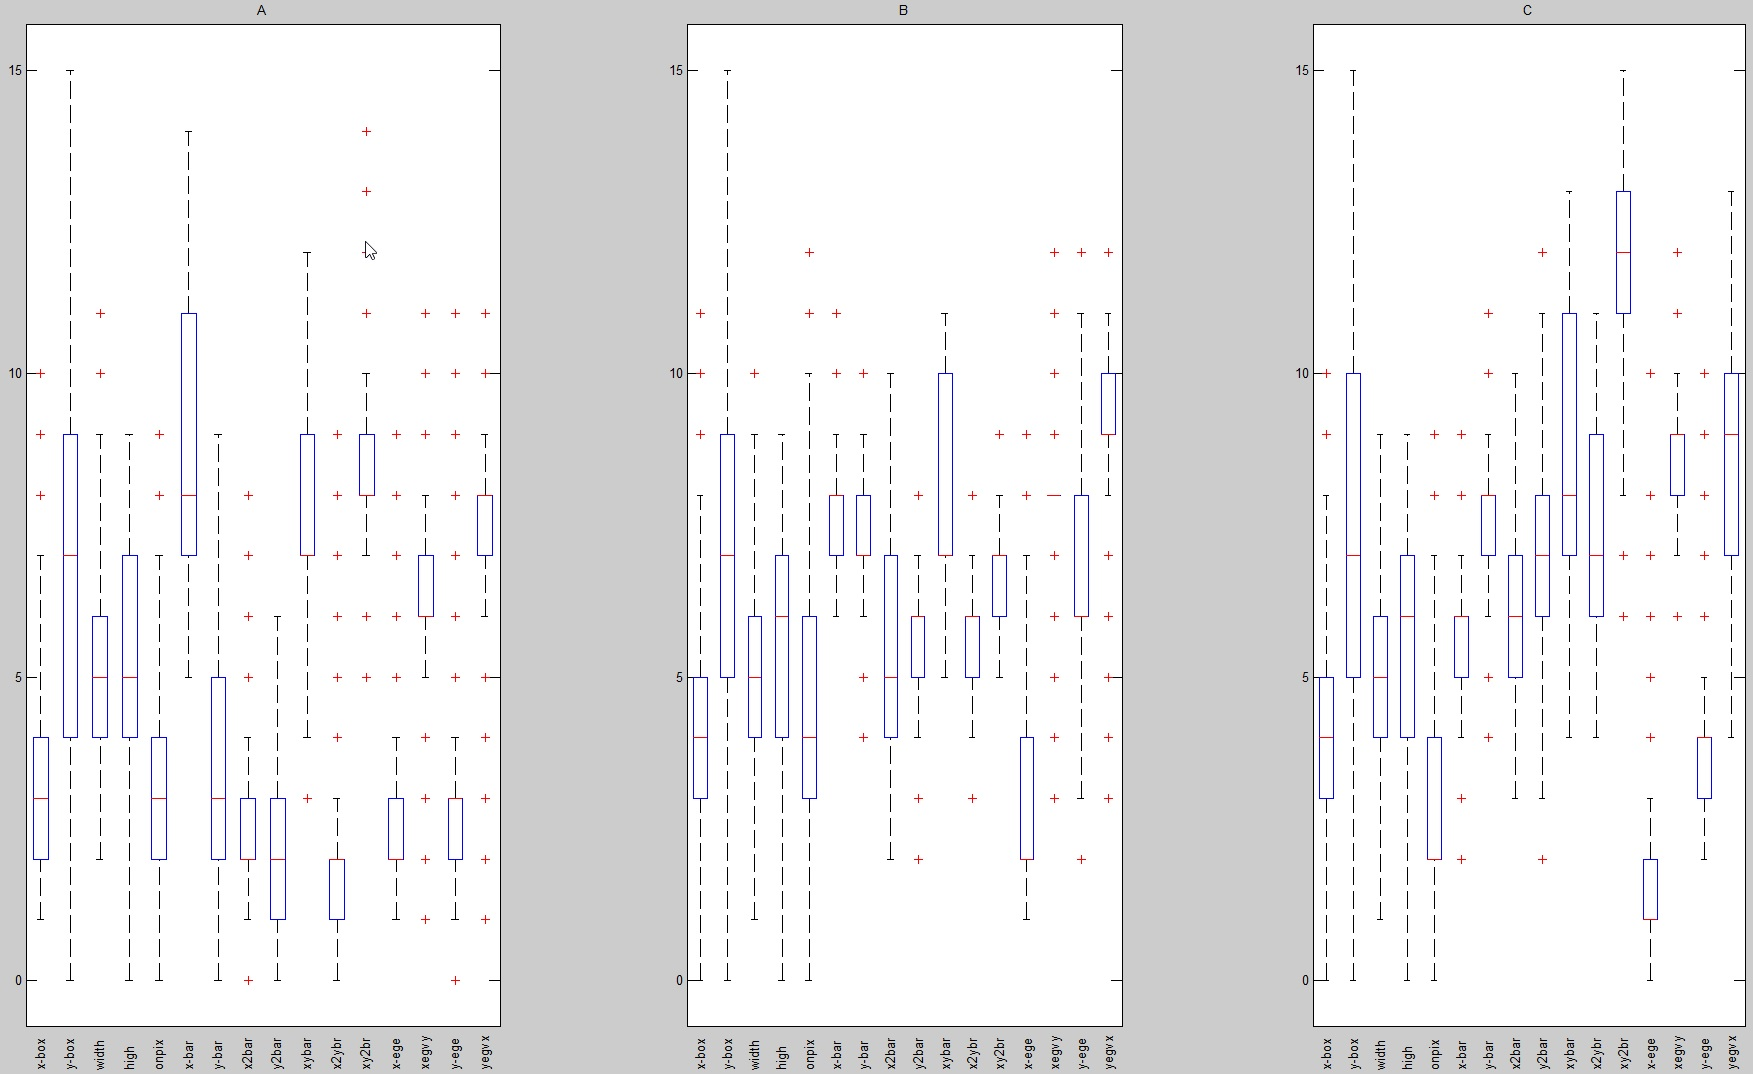
\includegraphics[width=0.9\textwidth]{figures/boxplot_perclass}
	\caption{Box plot for classes A,B,C of the data set}
	\label{fig:boxplot_perclass}
\end{figure}

\section*{Principal Component Analysis}
We applied principal component analysis (PCA) on our data set to convert
a set of our set of possibly correlated attributes into a set of values of
linearly uncorrelated variables called principal components. We normalized
the records in our data set by subtracting the mean and dividing by standard
deviation for each attribute. After that, we applied single value decomposition
to calculate the variation for every principal component (PC). \\

\subsection*{Variance}
Using a PCA technique we noticed that about 28\% of the variation is caused by
first PC, about 15\% by a second one, and about 12\% by the 3rd. It means that
first 3 principal components generate more than 50\% of the whole variance. 
\begin{figure}[!tbh]
	\centering
	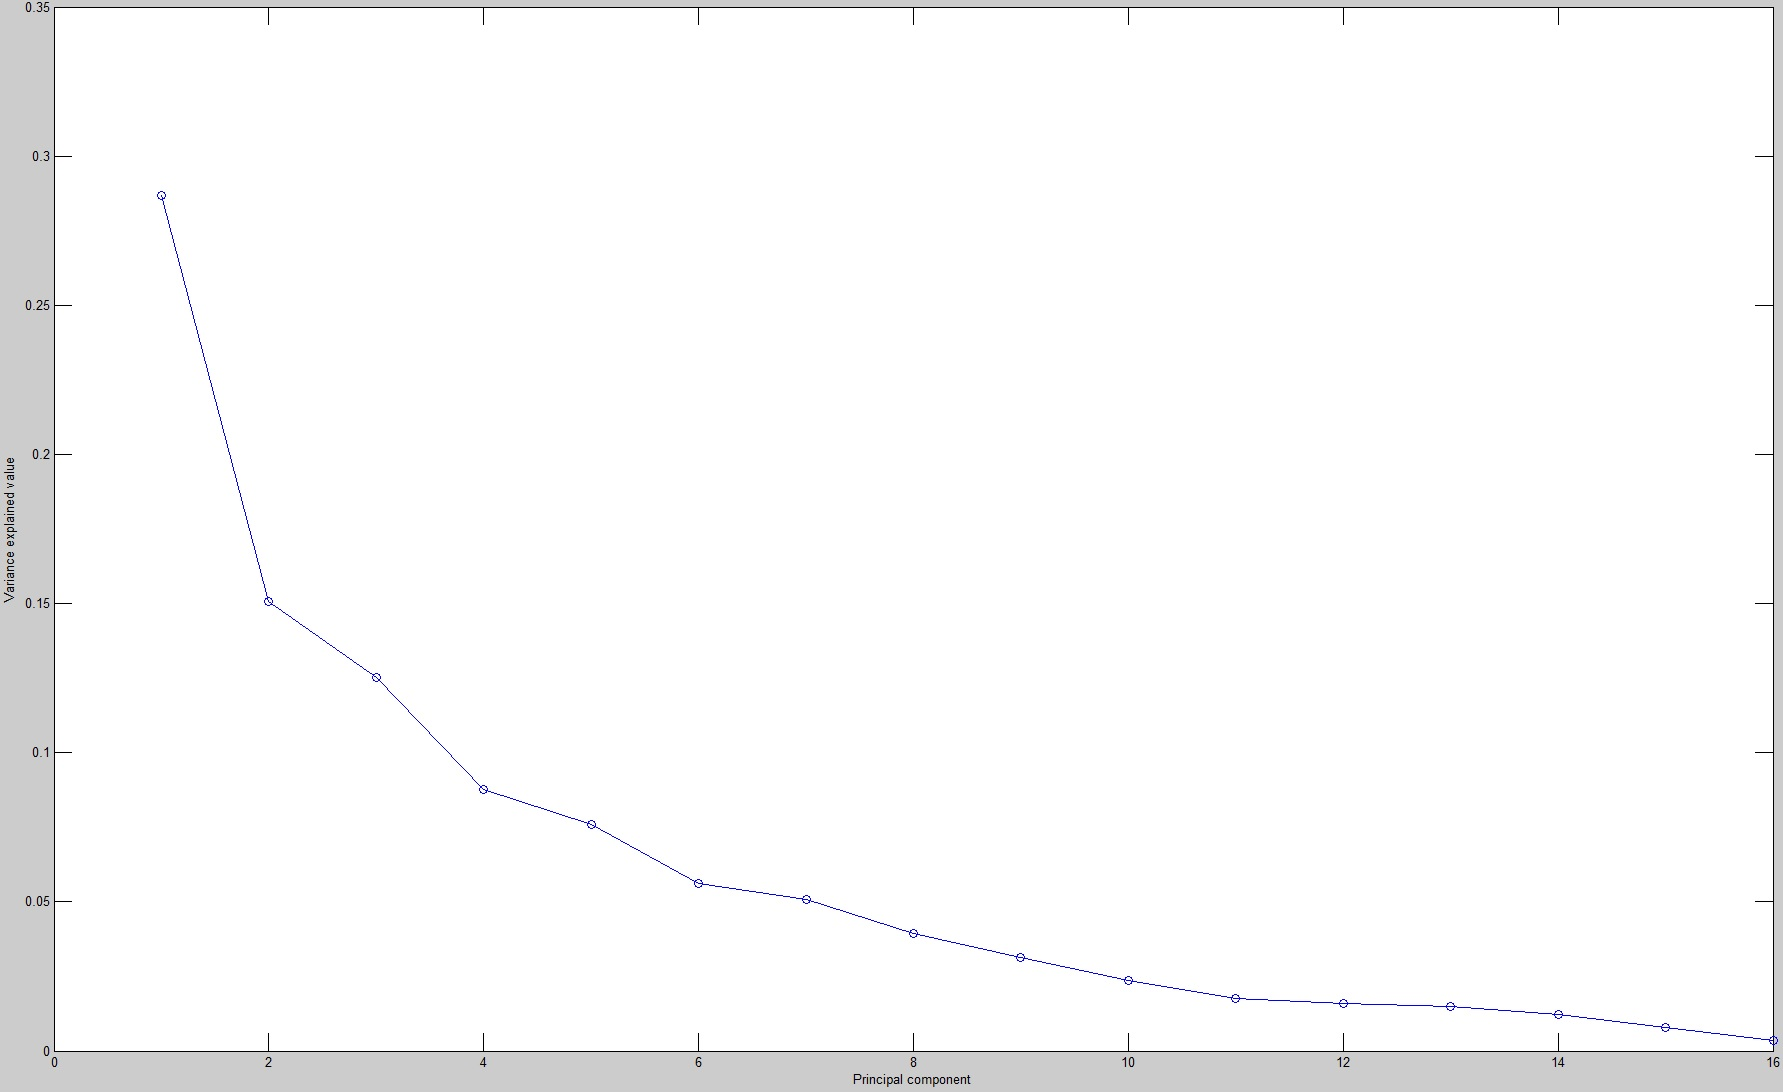
\includegraphics[width=1\textwidth]{figures/variance_perpc}
	\caption{Variance represented by each principal component}
	\label{fig:variance_perpc}
\end{figure} \\
The cumulative plot shows that over 9 principal components are needed to explain 
more than 90\% of the variation.
\begin{figure}[!tbh]
	\centering
	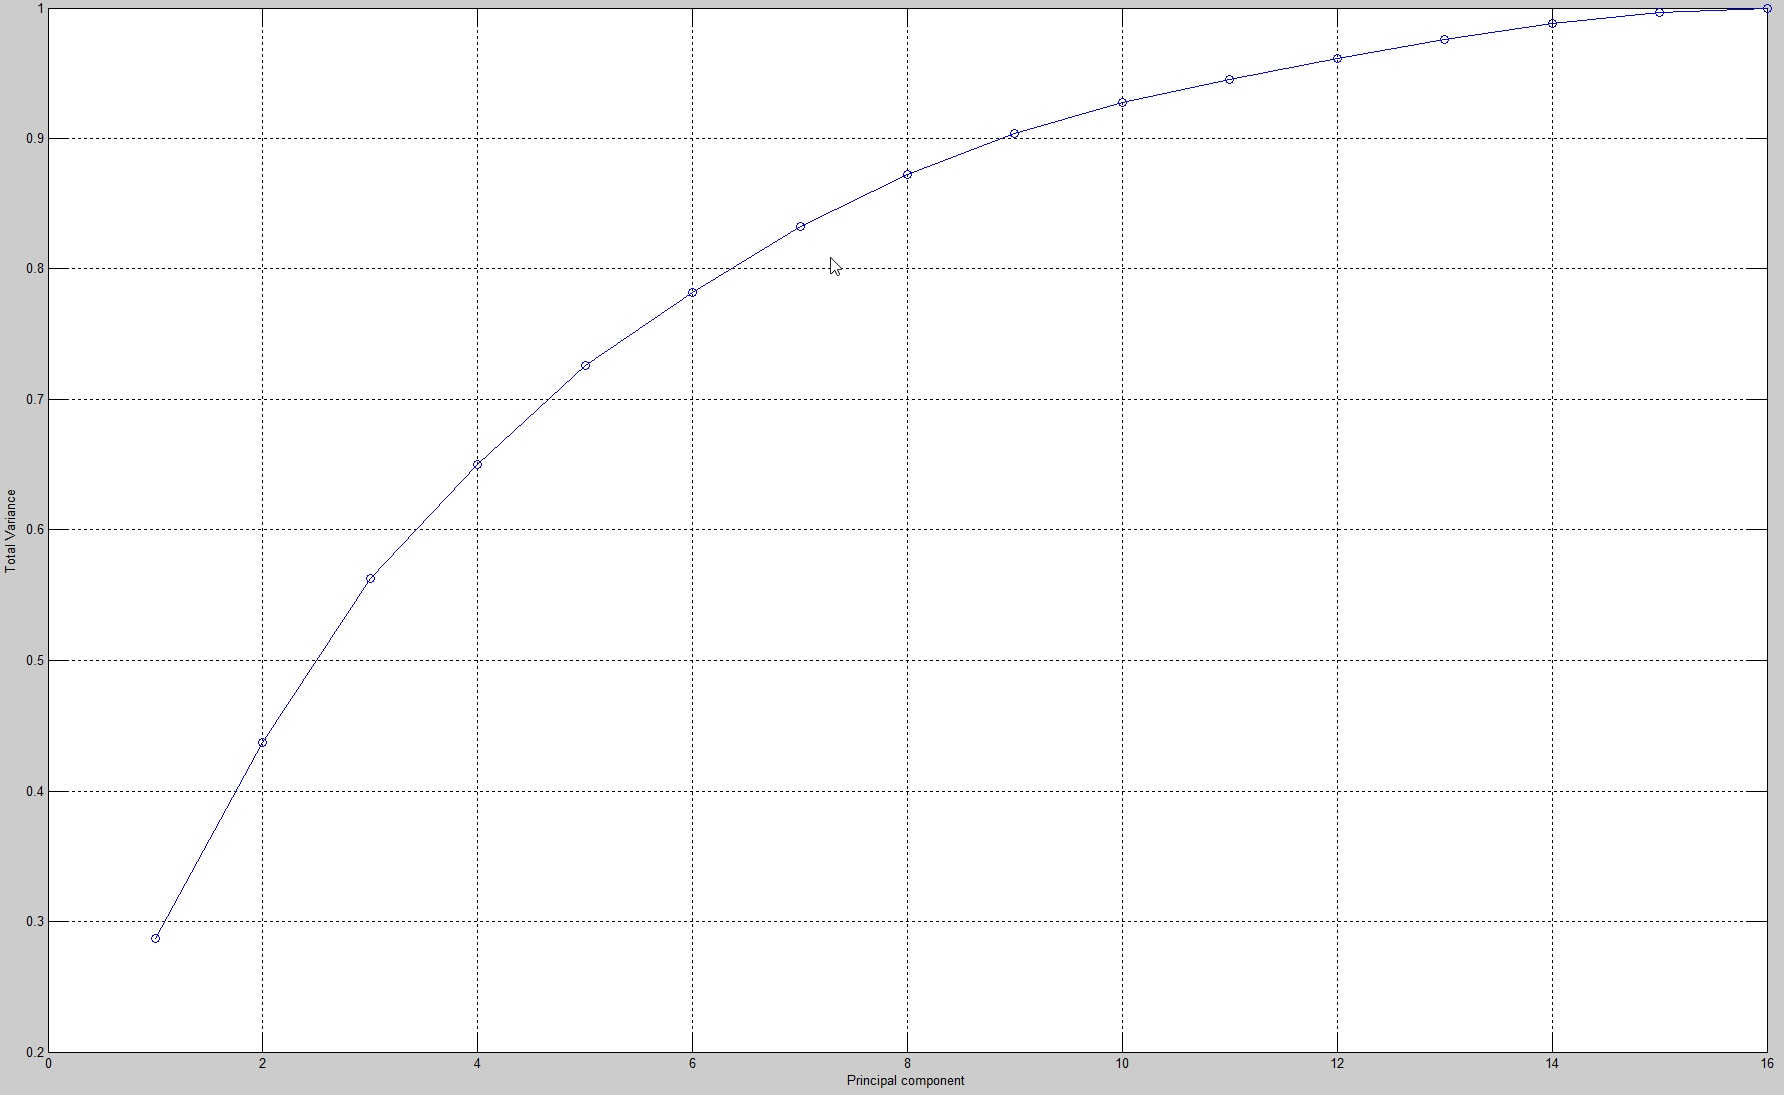
\includegraphics[width=1\textwidth]{figures/variance_cummulated}
	\caption{Cummulative variance for principal components}
	\label{fig:boxplot_cummulated}
\end{figure}
\clearpage
\subsection*{PCA - visualization}
Because of the fact that first 3 PC generate more than 50\% of the variance, we
decided to visualize records of our data set as a 3D points constructed of first
3 PC values. 
\begin{figure}[!tbh]
	\centering
	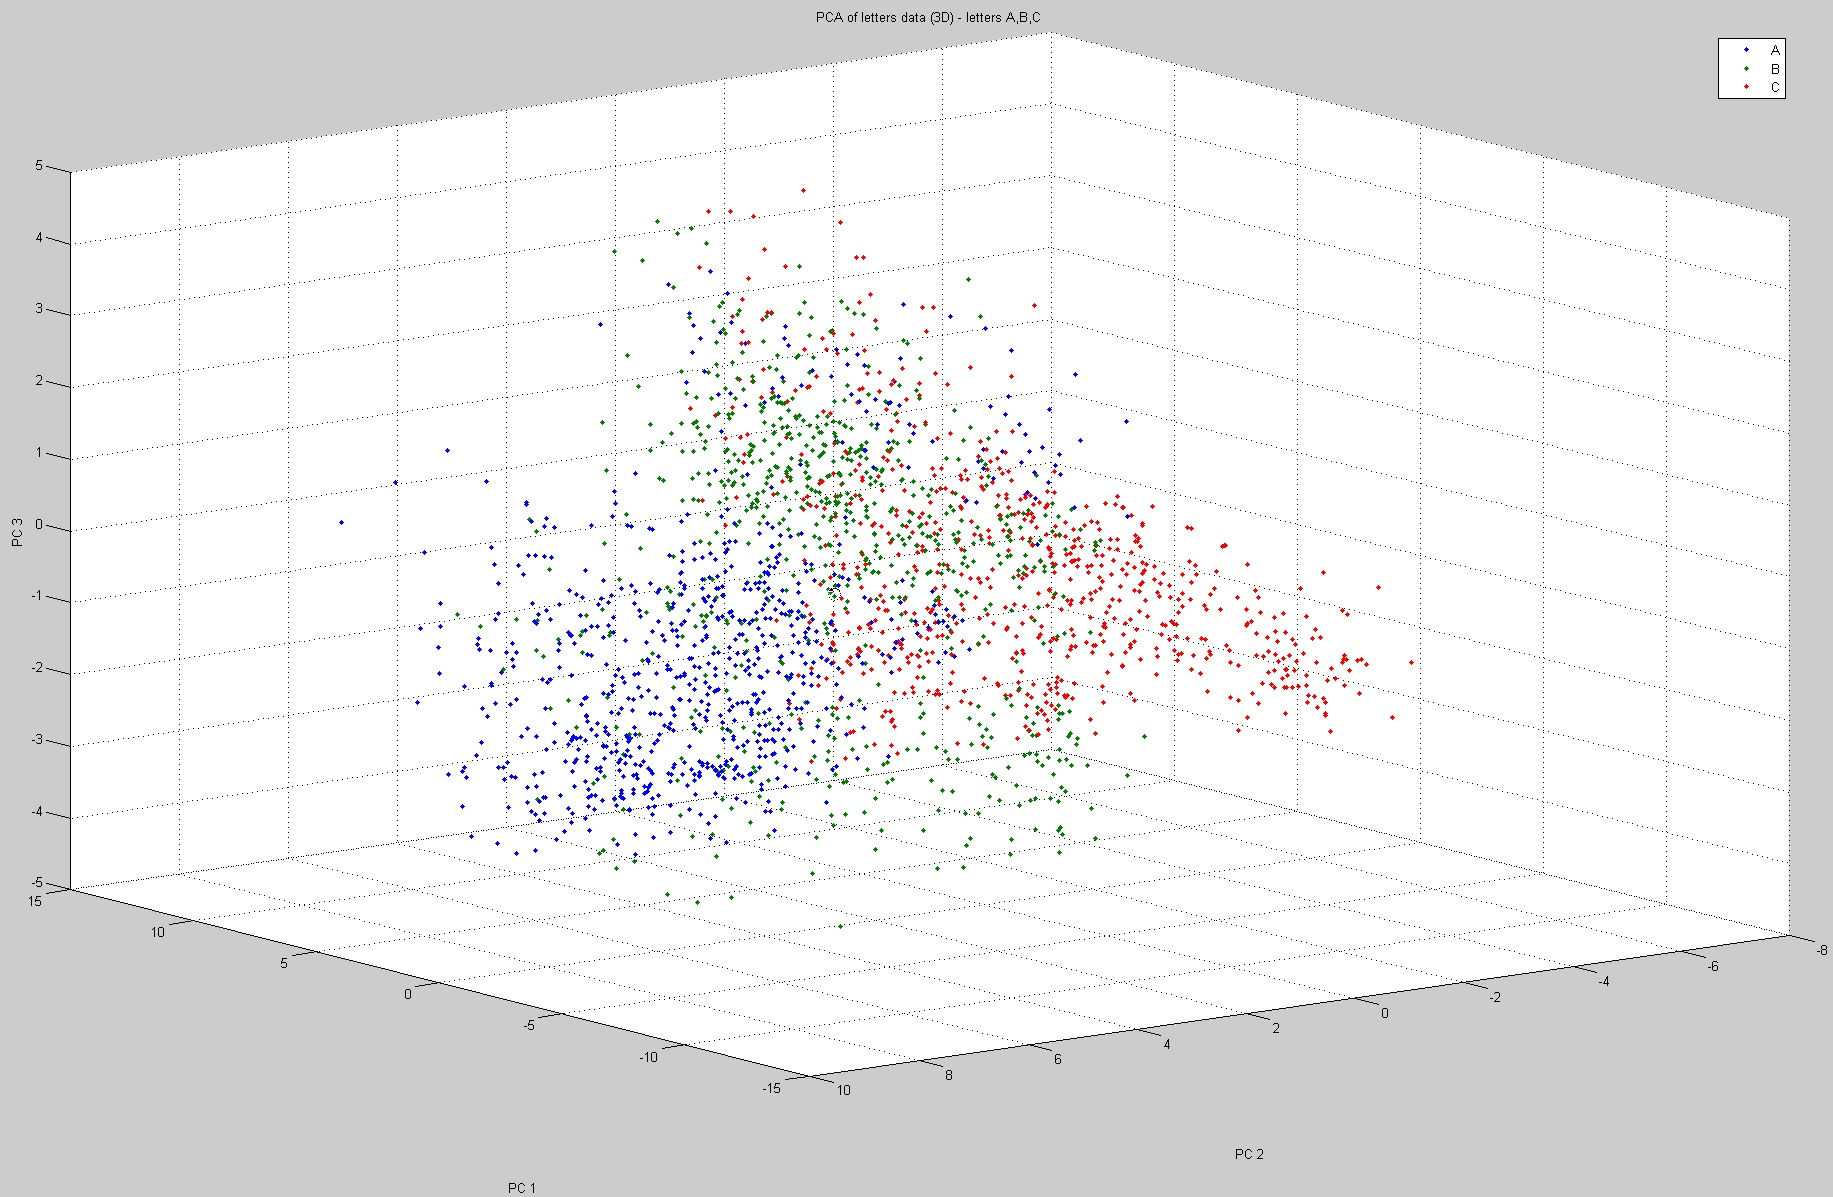
\includegraphics[width=0.75\textwidth]{figures/pca_points_abc_3D}
	\caption{Classes A,B and C represented by first 3 PC}
	\label{fig:pca_points_abc_3D}
\end{figure} 
Picture above shows a PCA visualization for first 3 PC of whole data set. 
In the picture below however, we can see a visualization only for first
three letters. We can see that it is possible with some probability 
to distinguish letters even using only first 3 PC's.
\begin{figure}[!tbh]
	\centering
	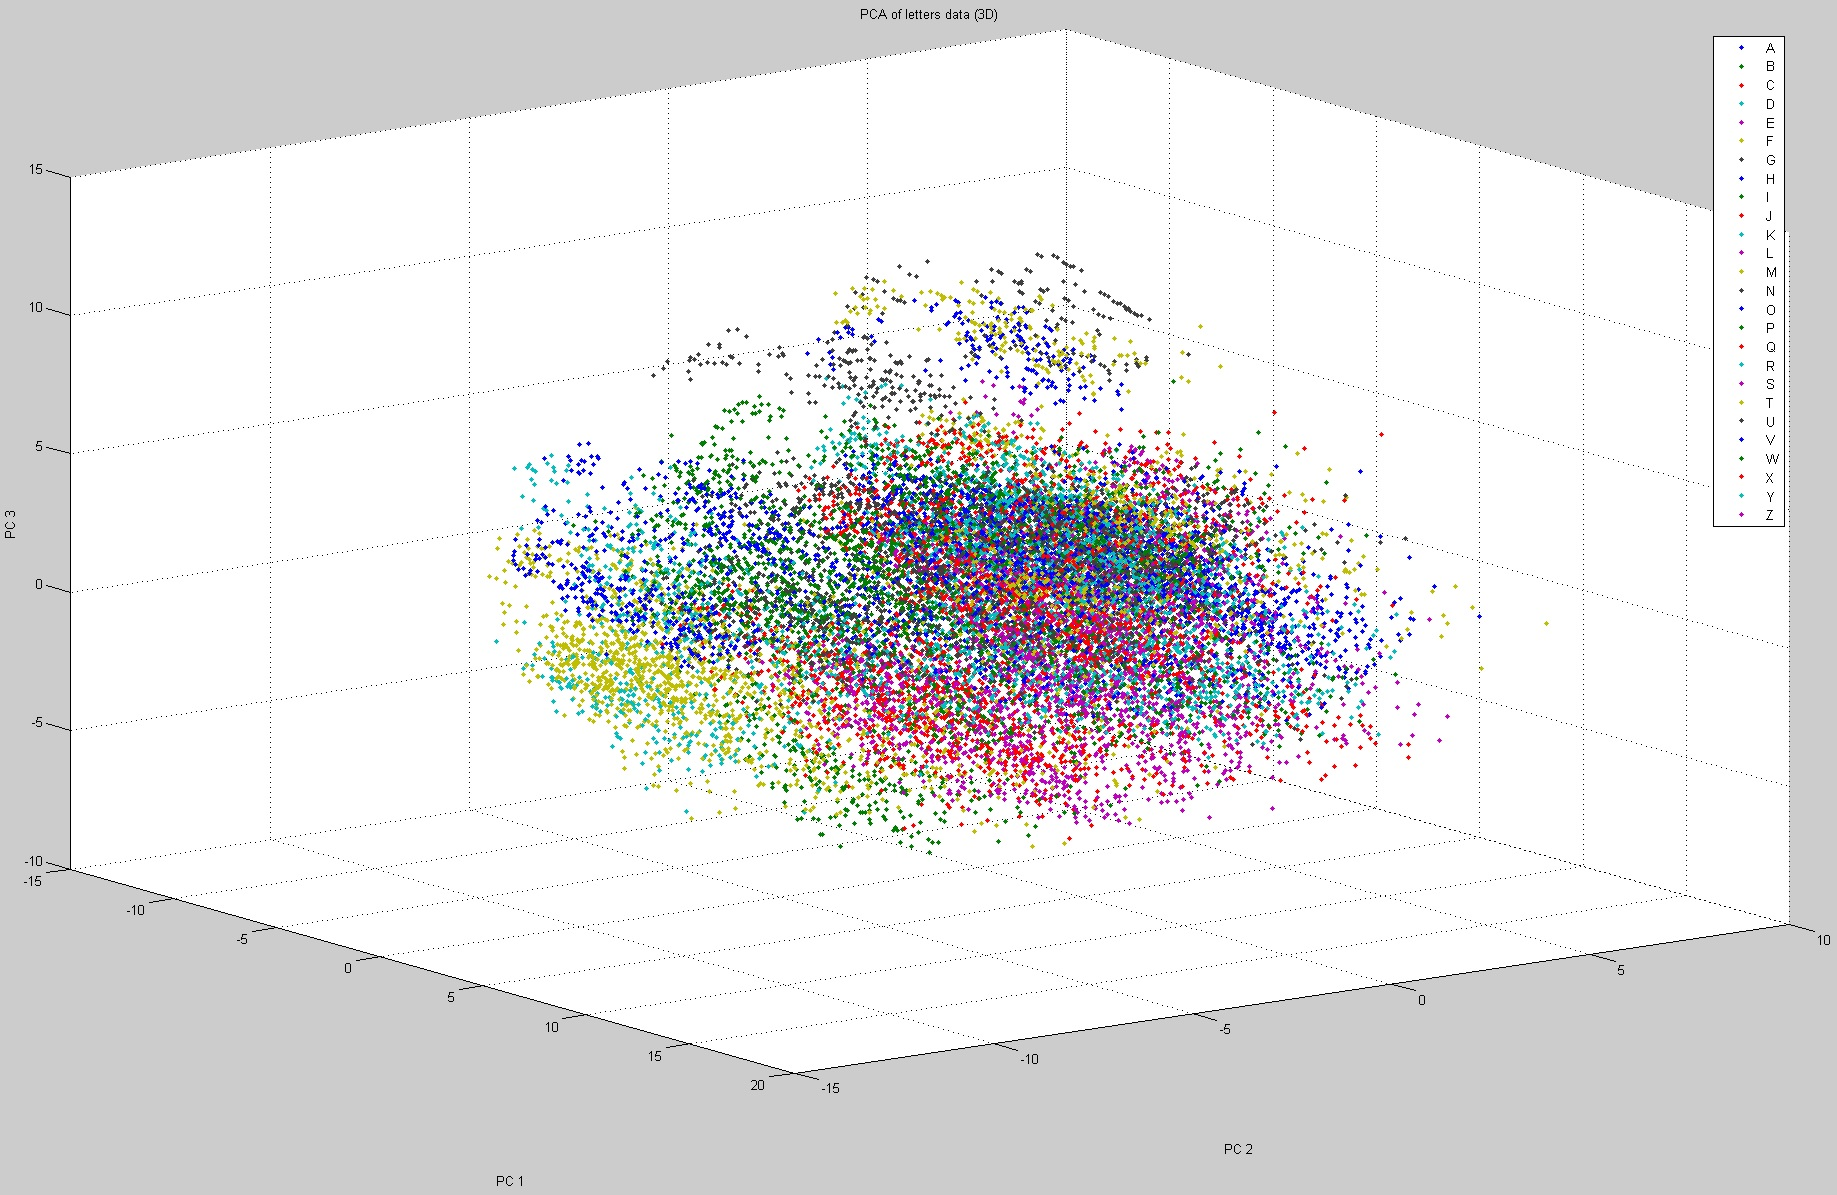
\includegraphics[width=0.75\textwidth]{figures/pca_points_all_3D}
	\caption{All the data set represented by first 3 PC}
	\label{fig:pca_points_all_3D}
\end{figure}